\section{Arquivos}
\begin{frame}
\frametitle{Arquivos}
\framesubtitle{}
\centering
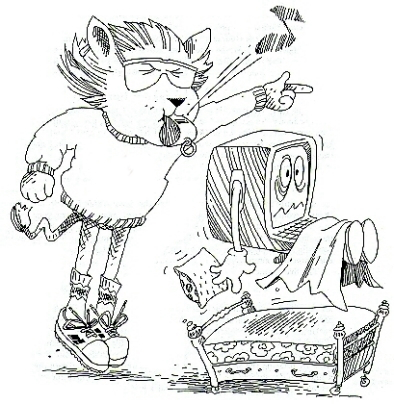
\includegraphics[width=0.4\linewidth,height=0.6\textheight,keepaspectratio]{figures/TexLionWhistle.jpg}
\end{frame}


\begin{frame}
\frametitle{Arquivos}

Arquivos são recursos computacionais para armazenar informações.

\pause 
\vspace{3ex}
O sistema de arquivos organiza e disponibiliza o acesso aos arquivos.

\pause
\vspace{3ex}
Nos sistemas modernos os arquivos são organizados em arranjos lineares de bytes.

\pause
\vspace{3ex}
O formato de um arquivo é definido pelo seu conteúdo. Muitos arquivos possuem um cabeçalho com metadados sobre si mesmo.
\end{frame}

\begin{frame}
\frametitle{Operações sobre arquivos}
\begin{itemize}%[<+->]
\item criar
\item alterar permissões de acesso e atributos
\item abrir
\item ler
\item escrever
\item fechar
\item apagar
\item trucar
\item acrescentar 
\end{itemize}
\end{frame}


\begin{frame}
\frametitle{Organização hierárquica}
\begin{minipage}{0.47\textwidth}
\dirtree{%
.1 spam.
.2 ham.
.2 eggs.
.3 more spam.
.3 dead parrots.
}
\end{minipage}
\hfill
\begin{minipage}{0.47\textwidth}
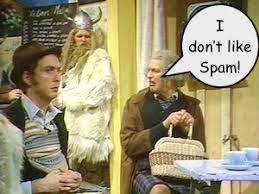
\includegraphics[width=\linewidth,height=0.5\textheight,keepaspectratio]{figures/mp-spam.jpg}
\end{minipage}
\end{frame}

\begin{frame}
\frametitle{Arquivo corrompido}
Dizemos que um arquivo é corrompido quando ele sofre alguma alteração de forma não possa mais ser lido (por software ou por humano). 
\end{frame}

\begin{frame}[fragile,allowframebreaks]
\frametitle{Codificação de arquivos}
\framesubtitle{Representação binária}
Arquivos são armazenados na forma binária no computador. 

\vspace{3ex}
Como exemplo, vamos analisar o arquivo \texttt{introducao.tex}.

\begin{footnotesize}
\begin{verbatim}
$ file introducao.tex 
introducao.tex: LaTeX document, UTF-8 Unicode text, with very long lines

$ ls -l introducao.tex
-rw-r--r-- 1 leoca leoca 9292 nov  1 14:10 introducao.tex
\end{verbatim}
\end{footnotesize}

\framebreak
\begin{footnotesize}
\begin{verbatim}
$ cat introducao.tex | xxd -b | head
00000000: 01011100 01100010 01100101 01100111 01101001 01101110  \begin
00000006: 01111011 01100110 01110010 01100001 01101101 01100101  {frame
0000000c: 01111101 00001010 01011100 01100110 01110010 01100001  }.\fra
00000012: 01101101 01100101 01110100 01101001 01110100 01101100  metitl
00000018: 01100101 01111011 01001111 00100000 01110001 01110101  e{O qu
0000001e: 01100101 00100000 11000011 10101001 00100000 01011100  e .. \
00000024: 01001100 01100001 01010100 01100101 01011000 01111011  LaTeX{
0000002a: 01111101 00111111 01111101 00001010 01011100 01100110  }?}.\f
00000030: 01110010 01100001 01101101 01100101 01110011 01110101  ramesu
00000036: 01100010 01110100 01101001 01110100 01101100 01100101  btitle
\end{verbatim}
\end{footnotesize}

\begin{footnotesize}
\begin{verbatim}
$ echo -n "TeX" | xxd
00000000: 5465 58                                  TeX

$ echo -n "TeX" | xxd -b
00000000: 01010100 01100101 01011000                             TeX
              T        e       X
hex          54       65      58 
dec          84      101      88
oct         124      144     130
\end{verbatim}
\end{footnotesize}
\end{frame}

\begin{frame}
\frametitle{Codificação de arquivos}
\framesubtitle{História}
  The Evolution of Character Codes, 1874-1968\\
  by Eric Fischer

  \vspace{2em}
  \url{https://github.com/ericfischer/ascii}
\end{frame}

\begin{frame}
\frametitle{Codificação de arquivos}
\framesubtitle{Código Morse - Samuel Morse e Alfred Vail (1837)}
        \centering
        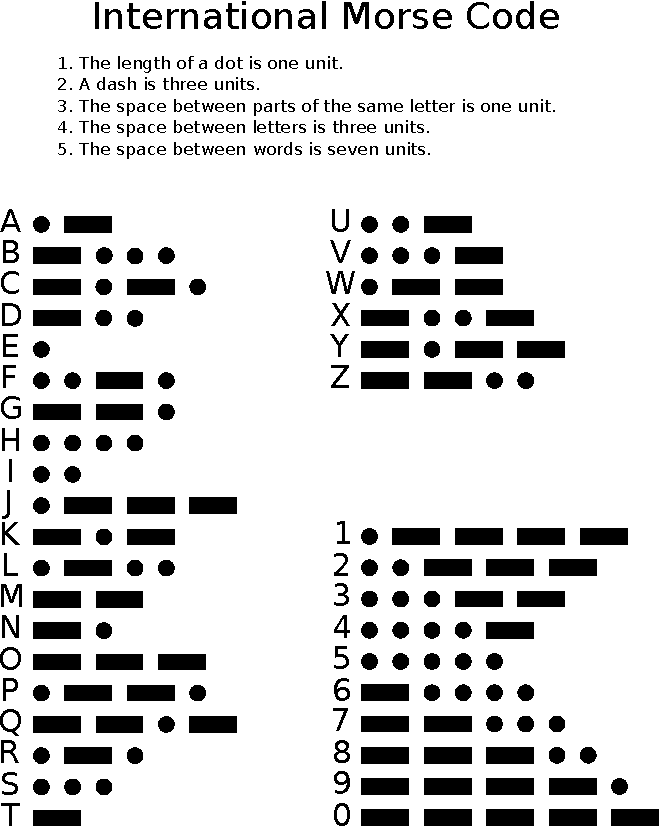
\includegraphics[width=0.3\textwidth,height=0.7\textheight,keepaspectratio]{figures/MorseCode.pdf} \hspace{3em}
        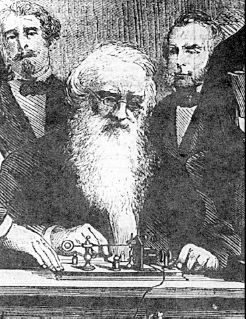
\includegraphics[width=0.3\textwidth,height=0.5\textheight,keepaspectratio]{figures/samuelmorse.jpg}
\end{frame}
\note{
Samuel Morse utilizou códigos de tamanho variável quando projetava o seu conhecido código telegráfico.
Samuel Morse havia sido comissionado em 1825 para pintar um retrato de Lafayette, em uma visita a Washington, DC.
Enquanto pintava, ele recebeu uma mensagem avisando que sua esposa estava muito doente.
Morse partiu imediatamente para sua casa em New Haven. Quando chegou sua esposa já havia sido enterrada.
Ele decidiu então se dedicar a explorar formas de comunicações a longa distância que fossem mais rápidas.

A primeira versão do código, desenvolvida por Morse durante uma viagem transatlântica em 1832,
era mais complexa do que a versão estabelecida em 1843. Mais tarde, Morse abandonou sua versão
em favor dos conhecidos pontos e traços desenvolvidos em conjunto com Alfred Vail.
Morse recebeu a patente do seu telégrafo com um único fio em 1847, sobrepujando o telégrafo
de múltiplos fios proposto por Cooke e Wheatstone, que havia sido patenteado em 1837.
}

\begin{frame}
\frametitle{Codificação de arquivos}
\framesubtitle{Código Baudot e Código Murray}
        \centering
        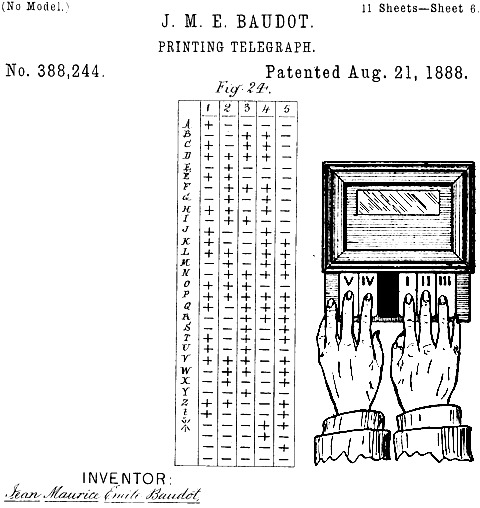
\includegraphics[width=0.3\textwidth,height=0.8\textheight,keepaspectratio]{figures/BaudotCode.png} \hspace{2em}
        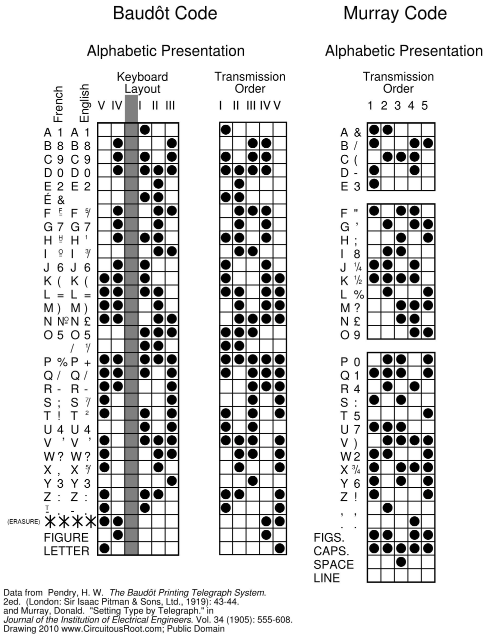
\includegraphics[width=0.35\textwidth,height=0.8\textheight,keepaspectratio]{figures/murraybaudot.png}
\end{frame}
\note{
Na França, Emile Baudout projetou seus sistema para o telégrafo em 1874.
Seu código foi baseado em código anterior desenvolvidos por 
Carl Friedrich Gauss e Wilhelm Weber em 1834.
Todos os símbolos possuem o mesmo comprimento, cinco. O projeto utilizava
um conjunto de fios funcionando de forma síncrona em um sistema de multiplexação,
onde o operador humano era responsável por realizar a divisão temporal e assim a sincronização.
Os códigos eram gerados por um aparelho com cinco teclas (similar às teclas de um piano),
sendo operado com duas mãos (dois dedos da mãos esquerda e três da mão direita).

Quando ordenados em alfabeticamente, as vogais e as consoantes, formam um código de Gray.

O código Baudout foi projetado para minimizar os movimentos da mão e dedos,
reduzindo assim a fadiga.
}\note{
O código de Baudout foi modificado por Donald Murray (1901) para ser utilizado
em um aparelho com teclado QWERTY. A mensagem é gravada em uma fita através de perfurações
e transmitida a partir desta fita perfurada. Deixou assim de existir a conexão direta entre
a mão do operador e a informação transmitida, não sendo mais necessário preocupar-se com a fadiga.
O objetivo passou então a ser simplificar o equipamento e minimizar seu desgaste, para tanto as
combinações com menos buracos foram utilizadas para designar caracteres mais frequentes
(ordem de freq. de occ. no inglês: e,t,a,o,i,n,s,h,r,d,l,c,u,m,w,f,g,y,p,b,v,k,j,x,q,z).


O código Murray também introduziu os caracteres de controle CR (carriage return) e
LF (line feed).
}


\begin{frame}
\frametitle{Codificação de arquivos}
\framesubtitle{Código Murray}
        \centering
        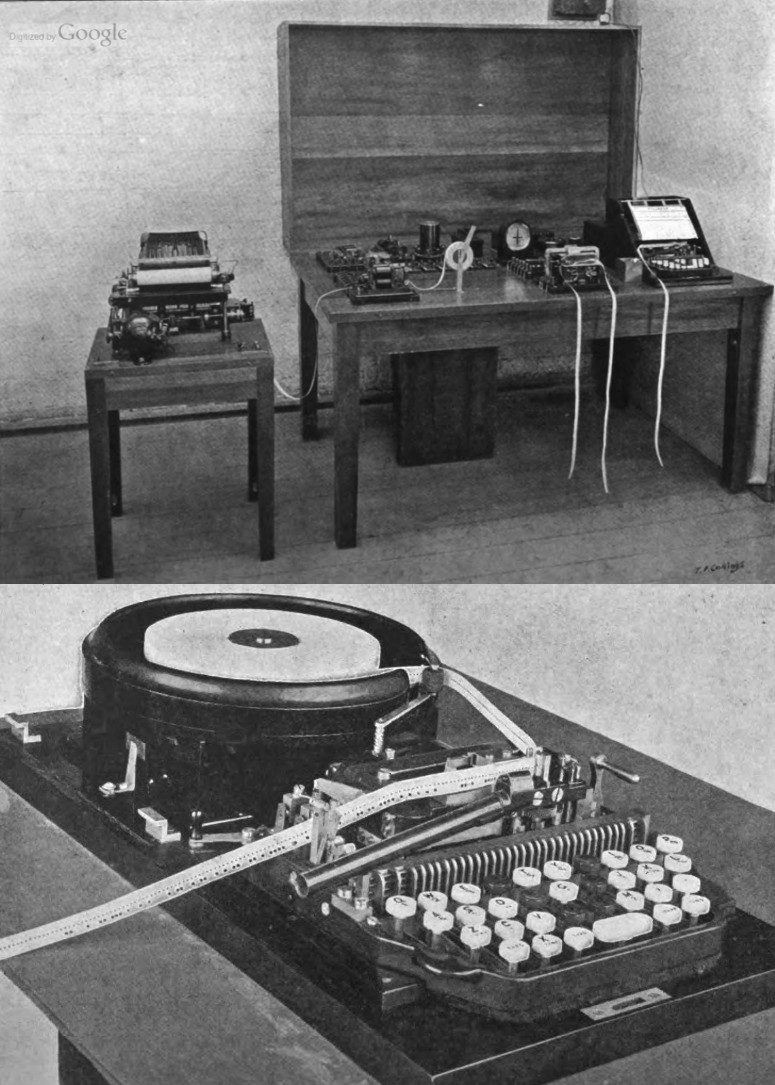
\includegraphics[width=0.35\textwidth,height=0.8\textheight,keepaspectratio]{figures/murrayapparatus.jpg} 
\end{frame}


\begin{frame}
\frametitle{Codificação de arquivos}
\framesubtitle{Western Union e ITA2}
   \begin{itemize}
   \item O código Murray foi adotado pelo Western Union com algumas modificações, sendo utilizado até os anos 50.
   \item Em 1924 o CCITT\footnote{O CCITT (International Telegraph and Telephone Consultative Committee) hoje conhecido
                                 como ITU-T (ITU Telecommunication Standardization Sector), um dos três setores do
                                 ITU (International Telecommunication Union) responsável pela definição de padrões em telecomunicações.}
         criou o ITA2 (international telegraph alphabet n. 2), baseado no código da Western Union.
   \item ITA2, também chamado de US TTY (American Teletypewriter code) foi a base para codificação em 5 bits dos Teletipos
         até o surgimento do código de 7 bits, ASCII em 1963.
   \end{itemize}
\end{frame}


\begin{frame}
\frametitle{Codificação de arquivos}
\framesubtitle{ASCII 1963 (7 bits)}
\centering
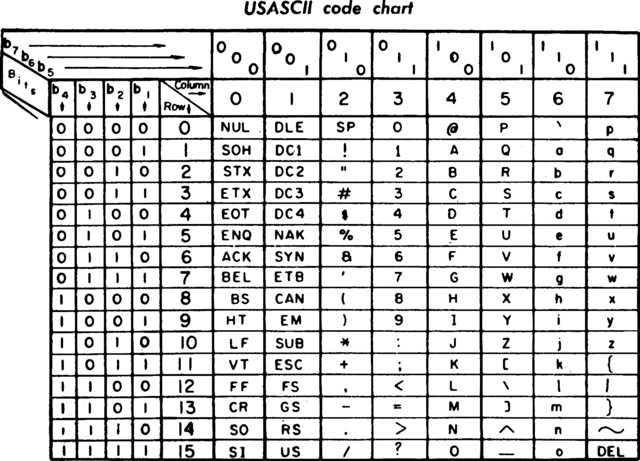
\includegraphics[width=0.65\textwidth,height=0.8\textheight,keepaspectratio]{figures/USASCII.png}
\end{frame}
\note{
\scriptsize
Foi desenvolvido pelo Comitê X3 da ASA (American Standards Association),
da qual faziam parte IBM (embora só passou a adotar o ASCII na década de 80),
AT\&T e sua subsidiária Teletype Corporation.

Os caracteres estão organizados de forma que os caracteres alfabéticos,
numéricos, matemáticos e de controle podem ser isolados através de uma
simples máscara binária.

O caractere A fica na posição $41_{\textmd{hex}}$ para ser compatível com o padrão
britânico. Os dígitos de 0 a 9 começam com $011$ e a sequência binária seguinte
corresponde ao valor binários de cada um deles, facilitando assim a conversão decimal-binário.

Os caracteres !"\#\$\%\&() foram adicionados à 2 coluna de forma a melhor se adequarem
à posição que ocupavam nos teclados das máquinas de escrever, de forma que a tecla \textit{shift}
corresponderia à uma simples mudança de um bit, assim facilitando a compatibilidade com as máquinas de escrever.

Foi cogitado utilizar um código com 8 bits, de forma que dois padrões de 4 bits
codificariam 2 dígitos. Isto iria requerer que fosse enviado sempre 8 bits.
Para minimizar custos, adotou-se 7 bits. Como as fitas perfuradas podiam armazenar
8 bits em cada posição, seria ainda possível utilizar um bit de paridade se desejado.
}


\begin{frame}
\frametitle{Codificação de arquivos}
\framesubtitle{Códigos de 8 bits}
  \begin{itemize}
  \item Extended ASCII 
  \item ISO/IEC 8859
  \item Windows-1252 (CP-1252)
  \end{itemize}

  Existem mais de 220 extensões DOS/Windows e 
  mais de 186 extensões EBCDIC (Extended Binary Coded Decimal Interchange Code),
  majoritariamente usado pela IBM.

  Dentre os padrões ISO o mais popular é o ISO 8859-1, também conhecido como ISO Latin 1,
  contendo a maioria dos caracteres utilizados pelas línguas da Europa Ocidental.
\end{frame}
\note{
A popularização do IBM System/360 e microprocessadores como o
Intel 8008, 8080 e 8086 acarretou na padronização do byte como uma unidade de 8 bits.
Endereçamento e armazenamento passaram a ser feitos em 8 bits, assim possibilitou a
extensão do ASCII utilizando o bit extra.
}

\begin{frame}
\frametitle{Codificação de arquivos}
\framesubtitle{Códigos Multi-Byte}
  \begin{itemize}
  \item Podem representar mais do que 256 caracteres.
  \item Alguns são extensões do ASCII (compatibilidade). Exemplo: UTF-8.
  \item UTF-16 não é uma extensão do ASCII pois os caracteres ASCII são armazenados em dois bytes, um deles igual a 0x00.
  \end{itemize}
\end{frame}

\begin{frame}[allowframebreaks]
\frametitle{Codificação de arquivos}
\framesubtitle{UFT-8}
  \begin{itemize}
  \item UTF-8: Unicode (ou Universal Coded Character Set) Transformation Format - 8-bit.
  \item Utiliza de 1 a 4 bytes.
  \item Capaz de representar até 1.112.064 pontos de codificação do Unicode.
  \item Compatibilidade reversa com ASCII (utiliza um único octeto com mesmo valor binário que o ASCII).
  \item Pontos de código mais usuais utilizam menos bytes que aqueles menos comuns.
  \item 128 caracteres ASCII necessitam de um byte (começando com 0). 
  \item 1920 caracteres utilizam 2 bytes para representar o restante do alfabeto latino (romano),
        grego, cirílico, copta, armênio, hebreu, arábico, siríaco, thaana e n'ko.
  \item Para as demais línguas são utilizados 3 bytes.
  \item 4 bytes para caracteres como símbolos matemáticos e emojis.
  \item O primeiro byte determina o número de bytes na sequência.
  \item UTF-8 foi apresentado em uma conferência em 1993. Em 2003 foi registrado pela RFC 3629 e 
        em 2008 tornou-se o padrão mais utilizado na internet.
  \item Criado por Ken Thompson e Rob Pike.
  \end{itemize}


  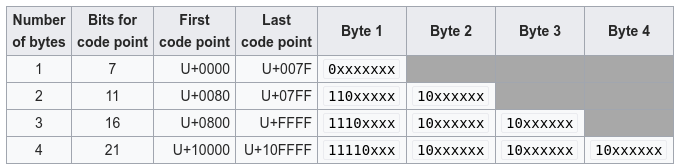
\includegraphics[width=0.85\textwidth,height=0.35\textheight,keepaspectratio]{figures/utf8bytes.png}

  {
  \centering
  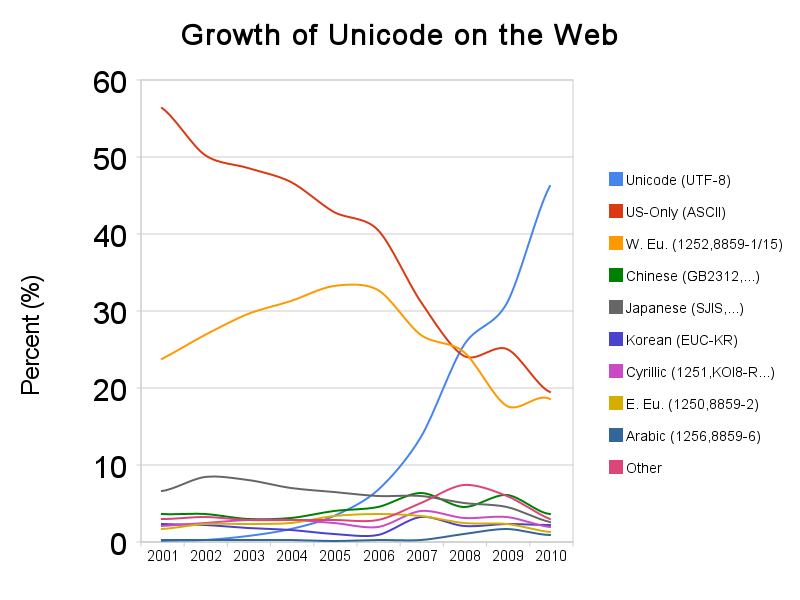
\includegraphics[width=0.55\textwidth,height=0.8\textheight,keepaspectratio]{figures/unicodeweb.png} 
  }
  \footnotesize{googleblog: \url{https://googleblog.blogspot.com.br/2010/01/unicode-nearing-50-of-web.html}}
  

  {
  \centering
  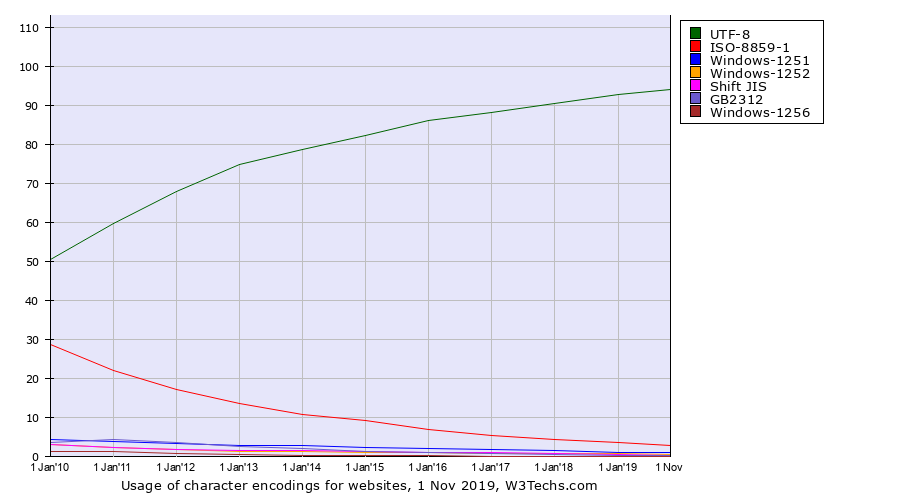
\includegraphics[width=0.6\textwidth,height=0.8\textheight,keepaspectratio]{figures/w3usage.png}
  }
  \footnotesize{W3Techs: \url{https://w3techs.com/technologies/history_overview/character_encoding/ms/y}}
\end{frame}

\begin{frame}
\frametitle{Codificação de arquivos}
\framesubtitle{Unicode}
  O Unicode é uma padrão para a industria de computadores para estabelecer uma 
  codificação, representação e manipulação consistente de textos utilizados por grande parte dos
  sistemas de escrita do mundo.

  A última versão do Unicode possui 136.755 caracteres cobrindo 139 escritas modernas e antigas, 
  e também outros conjuntos símbolos utilizados na comunicação humana (por exemplo, símbolos matemáticos
  e emojis).

  O Unicode é mantido pelo Consórcio do Unicode, criado em 1991, cujos membros incluem Adobe, Apple, Google, Huawei, IBM,
  Microsoft, Oracle, Yahoo! e SAP.
\end{frame}

\begin{frame}[allowframebreaks]
\frametitle{Codificação de arquivos}
\framesubtitle{Extremidade (\textit{endianness})}
  O termo \textbf{extremidade} (endianness) refere-se a ordem utilizada para armazenar/ler os bytes ou bits de dados.

  Byte 
  \hrule
  \begin{description}
  \item[big-endian]: extremidade maior primeiro -  Motorola (famílias 6800 e 68000), PowerPC (Apple).
  \item[little-endian]: extremidade menor primeiro - Intel (x86), AMD, Zilog (Z80), MOS Technology (6502), DEC (VAX e PDP-11).
  \end{description}

  Bit
  \hrule
  \begin{description}
  \item[LSB 0]: a numberação dos bits inicia-se pelo menos significante - SPARC e Motorola 68000.
  \item[MSB 0]: a numberação dos bits inicia-se pelo mais significante - S/390, PowerPC e PA-RISC (recomendada pela RfC).
  \end{description}

  \framebreak
  \begin{itemize}
  \item Lilliput - Viagens de Gulliver (Jonathan Swift).
  \item Unicode - marcador BOM (Byte Order Mark) - ponto de representação \texttt{U+FEFF}.
  \item No UTF-8 o marcador BOM é representado pela sequência de 3 octetos: \texttt{0xEF,0xBB,0xBF} (1110 1111 1011 1011 1011 1111).
  \item Extremidade (byte) é irrelevante para o padrão UTF-8 e portanto o marcador BOM é desnecessário.
  \item No padrão UTF-16 a sequência de bytes \texttt{0xFE,0xFF} indica ordenação \textit{big-endian} e a sequência \texttt{0xFF,0xFE}
        indica a ordenação \textit{little-endian}.
  \end{itemize}

  \hfill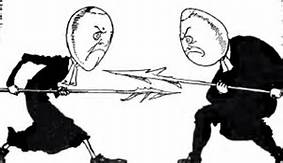
\includegraphics[width=0.2\textwidth,height=0.3\textheight,keepaspectratio]{figures/lilliputwar.jpg}
\end{frame}
\note{
As CPUs que utilizam \textit{little-endian} usualmente usam o `LSB 0', enquanto
as CPUs que utilizam \textit{big-endian} utilizam ambas padronizações.
O estilo recomendado pela RfC (Request for Comments) é `MSB 0'.
Algumas arquiteturas, como SPARC e Motorola 68000 utilizam `LSB 0', enquanto
S/390, PowerPC e PA-RISC utilizam `MSB 0'.
}
\note{
``O termo em inglês para uma forma de \emph{endianness}, \emph{big-endian}, é uma referência às Viagens de Gulliver: 
em Lilliput houve uma guerra civil, entre os que preferiam quebrar os ovos cozidos pelo lado maior (big-endians) 
contra quem preferia quebrar os ovos cozidos pelo lado menor. Este conflito, por sua vez, era uma paródia 
entre as diferenças entre católicos e protestantes a respeito da transubstanciação.'' (Wikipedia)
\url{https://pt.wikipedia.org/wiki/Extremidade\_(ordena\\\%C3\\\%A7\\\%C3\\\%A3o)}
}

\begin{frame}[fragile]
\frametitle{Determinando a codificação}

O comando \texttt{file} do Linux/Unix/OS X/macOS tenta `adivinhar' qual é a codificação do arquivo.

\begin{lstlisting}[language=bash, label=lst-filecod, caption={Determinando o tipo de codificação de um arquivo.}, postbreak=\mbox{$\hookrightarrow$\space}, basicstyle=\fontsize{8}{10}\selectfont\ttfamily]
$ file -i arquivo.csv
arquivo.csv: application/csv; charset=us-ascii
$ file -i arquivo.xls 
arquivo.xls: text/plain; charset=utf-16le
$ file -i imagem.png 
imagem.png: image/png; charset=binary
$ file -i imagem.jpg 
imagem.jpg: image/jpeg; charset=binary
\end{lstlisting}
\end{frame}

\begin{frame}[fragile]
\frametitle{Convertendo o tipo de codificação}
O comando \texttt{iconv} converte um tipo de codificação de caracteres em outro tipo. Faz a conversão entre 1179 tipos de codificação.
\begin{lstlisting}[language=bash, label=lst-iconv, caption={Convertendo o tipo de codificação de um arquivo.}, postbreak=\mbox{$\hookrightarrow$\space}, basicstyle=\fontsize{8}{10}\selectfont\ttfamily]
$ iconv -f ISO-8859-1 -t ASCII arquivo.txt > arquivo_ascii.txt
$ iconv -f ISO-8859-1 -t ASCII//TRANSLIT input.file -o out.file
$ iconv -f ISO-8859-1 -t UTF-8//IGNORE input.file -o out.file
\end{lstlisting}
\end{frame}

\begin{frame}[fragile]
\frametitle{Exemplo - declaração de codificação em um HTML}
\begin{lstlisting}[language=html, label=lst-htmlenc, caption={Documento HTML.}, postbreak=\mbox{$\hookrightarrow$\space}, basicstyle=\fontsize{8}{10}\selectfont\ttfamily]
<!DOCTYPE html>
<html lang="en">
<head>
<meta http-equiv="Content-Type" content="text/html; charset=utf-8"/>
\end{lstlisting}
\end{frame}


\begin{frame}[fragile]
\frametitle{A traição dos nomes}
\begin{figure}[h]
\centering
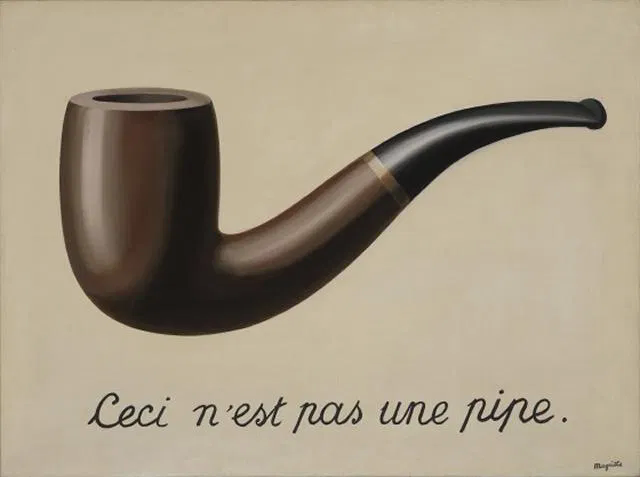
\includegraphics[width=0.5\textwidth,height=0.7\textheight,keepaspectratio]{figures/magritte.png}
\caption{\emph{La trahison des images}, René Magritte (1929).}
\label{fig-magritte}
\end{figure}
\end{frame}
\note{
``Este quadro, uma das obras-primas surrealistas do artista, está atualmente no Museu de Arte do Condado de Los Angeles (LACMA), Califórnia (...)
Fortemente influenciado pela psicologia freudiana, o surrealismo representou uma reação contra o "racionalismo". A Traição das Imagens desafia a convenção linguística de identificar uma imagem de algo como a coisa em si. (...) René Magritte nega aquilo que estamos a ver. A uma primeira análise, o significado desta negação torna-se claro, pois aquilo que estamos a ver não é um cachimbo verdadeiro, mas sim a representação de um cachimbo. Deparamo-nos com um desafio àquilo que se convencionou chamar de "cachimbo", pois a nossa imagem de cachimbo está negada. Magritte como que esvaziou de sentido aquilo que entendemos como sendo a palavra "cachimbo". Não podemos identificar esta representação com aquilo que é o objeto, gerando-se, assim, um conflito de mensagens.''(\hrefcolor{https://pt.wikipedia.org/wiki/A_Trai\%C3\%A7\%C3\%A3o_das_Imagens}{Wikipedia - A Traição das Imagens})
}


\begin{frame}[allowframebreaks]
\frametitle{Formatos de arquivos}
\begin{description}
\item[ASCII, UTF-8](\texttt{.txt}) texto puro 
\item[MS Word](\texttt{.doc} e \texttt{.docx}) formato binário e XML estruturado, respectivamente
\item[DjVu](\texttt{.djvu}) formato utilizado principalmente para documentos escaneados
\item[HTML](\texttt{.html} ou \texttt{.htm}) páginas Web (padrão ISO)
\item[PDF](\texttt{.pdf}) padrão aberto\footnote{O padrão PDF passou a ser um padrão aberto em 1 de julho de 2008.} para troca de documentos (ISO 32000)
\item[PostScript](\texttt{.ps}) linguagem de descrição de página
\item[SVG](\texttt{.svg}) gráficos vetoriais escalonáveis
\item[TeX](\texttt{.tex}) arquivos texto para produção de documentos utilizando \TeX{}
\item[BMP](\texttt{.bmp}) imagens Bitmap do Windows
\item[GIF](\texttt{.gif}) imagens rasterizadas 
\item[PNG](\texttt{.png}) imagens rasterizadas (formato aberto)
\item[JPEG](\texttt{.jpg} ou \texttt{.jpeg}) formato para imagens rasterizadas (compressão com perdas)
\item[WAV](\texttt{.wav}) Microsoft Wave (sem compressão)
\item[FLAC](\texttt{.flac}) formato de áudio com compressão sem perdas
\item[MP3](\texttt{.mp3}) formato de áudio com compressão com perdas (patenteado)
\item[OGG](\texttt{.ogg}) formato aberto de áudio com compressão com perdas 
\end{description}
\end{frame}

\begin{frame}[fragile,allowframebreaks]
\frametitle{Exemplo \texttt{.docx}}

\begin{figure}[h]
\centering
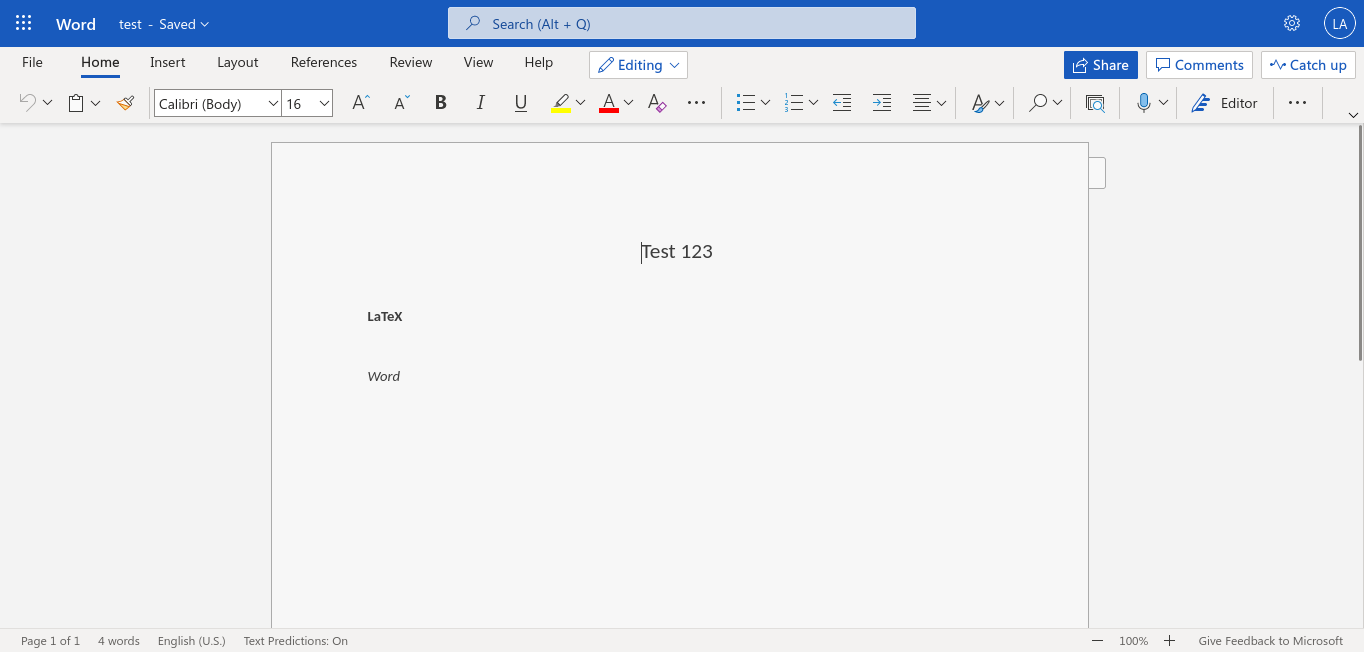
\includegraphics[width=0.8\textwidth,height=0.8\textheight,keepaspectratio]{figures/test-word.png}
\caption{Documento exemplo criado no Office 365.}
\label{fig-word-test}
\end{figure}

\framebreak

\begin{lstlisting}[language=bash, label=lst-docx, caption={Conteúdo do arquivo \texttt{.docx} exemplo. Visualização com \texttt{vim}.}, postbreak=\mbox{$\hookrightarrow$\space}, basicstyle=\fontsize{6}{8}\selectfont\ttfamily]
" zip.vim version v28
" Browsing zipfile /tmp/test.docx
" Select a file with cursor and press ENTER

[Content_Types].xml
_rels/.rels
word/theme/theme1.xml
word/settings.xml
word/fontTable.xml
word/webSettings.xml
docProps/app.xml
docProps/core.xml
word/styles.xml
word/document2.xml
word/_rels/document2.xml.rels
\end{lstlisting}

\framebreak

\begin{lstlisting}[language=xml, label=lst-docx-1, caption={Conteúdo do arquivo \texttt{word/document2.xml}}, postbreak=\mbox{$\hookrightarrow$\space}, basicstyle=\fontsize{6}{8}\selectfont\ttfamily]
<?xml version="1.0" encoding="utf-8" standalone="yes"?><w:document xmlns:wpc="http://schemas.microsoft.com/office/word/2010/wordprocessingCanvas" xmlns:mc="http://schemas.openxmlformats.org/markup-compatibility/2006" xmlns:o="urn:schemas-microsoft-com:office:office" xmlns:r="http://schemas.openxmlformats.org/officeDocument/2006/relationships" xmlns:m="http://schemas.openxmlformats.org/officeDocument/2006/math" xmlns:v="urn:schemas-microsoft-com:vml" xmlns:wp14="http://schemas.microsoft.com/office/word/2010/wordprocessingDrawing" xmlns:wp="http://schemas.openxmlformats.org/drawingml/2006/wordprocessingDrawing" xmlns:w10="urn:schemas-microsoft-com:office:word" xmlns:w="http://schemas.openxmlformats.org/wordprocessingml/2006/main" xmlns:w14="http://schemas.microsoft.com/office/word/2010/wordml" xmlns:w15="http://schemas.microsoft.com/office/word/2012/wordml" xmlns:wpg="http://schemas.microsoft.com/office/word/2010/wordprocessingGroup" xmlns:wpi="http://schemas.microsoft.com/office/word/2010/wordprocessingInk" xmlns:wne="http://schemas.microsoft.com/office/word/2006/wordml" xmlns:wps="http://schemas.microsoft.com/office/word/2010/wordprocessingShape" mc:Ignorable="w14 w15 wp14"><w:body><w:p w:rsidP="4FDD56AD" w14:paraId="2C078E63" xmlns:wp14="http://schemas.microsoft.com/office/word/2010/wordml" wp14:textId="19C3A7FB"><w:pPr><w:jc w:val="center" /><w:rPr><w:b w:val="0" /><w:bCs w:val="0" /><w:sz w:val="32" /><w:szCs w:val="32" /></w:rPr></w:pPr><w:bookmarkStart w:name="_GoBack" w:id="0" /><w:bookmarkEnd w:id="0" /><w:r w:rsidRPr="4FDD56AD" w:rsidR="79861D53"><w:rPr><w:b w:val="0" /><w:bCs w:val="0" /><w:sz w:val="32" /><w:szCs w:val="32" /></w:rPr><w:t>Test 123</w:t></w:r></w:p><w:p w:rsidR="4FDD56AD" w:rsidP="4FDD56AD" w:rsidRDefault="4FDD56AD" w14:paraId="2700AB13" w14:textId="40AAB38F"><w:pPr><w:pStyle w:val="Normal" /></w:pPr></w:p><w:p w:rsidR="79861D53" w:rsidP="4FDD56AD" w:rsidRDefault="79861D53" w14:paraId="53B87EDE" w14:textId="05C1A8EF"><w:pPr><w:pStyle w:val="Normal" /></w:pPr><w:r w:rsidRPr="4FDD56AD" w:rsidR="79861D53"><w:rPr><w:b w:val="1" /><w:bCs w:val="1" /></w:rPr><w:t>LaTeX</w:t></w:r></w:p><w:p w:rsidR="4FDD56AD" w:rsidP="4FDD56AD" w:rsidRDefault="4FDD56AD" w14:paraId="521FC589" w14:textId="672BCEF3"><w:pPr><w:pStyle w:val="Normal" /></w:pPr></w:p><w:p w:rsidR="79861D53" w:rsidP="4FDD56AD" w:rsidRDefault="79861D53" w14:paraId="65FC53F7" w14:textId="703EA904"><w:pPr><w:pStyle w:val="Normal" /></w:pPr><w:r w:rsidRPr="4FDD56AD" w:rsidR="79861D53"><w:rPr><w:i w:val="1" /><w:iCs w:val="1" /></w:rPr><w:t>Word</w:t></w:r></w:p><w:sectPr><w:pgSz w:w="12240" w:h="15840" w:orient="portrait" /><w:pgMar w:top="1440" w:right="1440" w:bottom="1440" w:left="1440" w:header="720" w:footer="720" w:gutter="0" /><w:cols w:space="720" /><w:docGrid w:linePitch="360" /></w:sectPr></w:body></w:document>
\end{lstlisting}

\end{frame}

\begin{frame}[fragile,allowframebreaks]
\frametitle{Exemplo imagem PNM}


\includegraphics[width=0.1\textwidth,height=0.1\textheight,keepaspectratio]{figures/pikachu.png}

\begin{lstlisting}[language=bash, label=lst-pnm-ascii, caption={Arquivo PNM ASCII.}, postbreak=\mbox{$\hookrightarrow$\space}, basicstyle=\fontsize{6}{8}\selectfont\ttfamily]
P3
# Created by GIMP version 2.10.18 PNM plug-in
64 64
255 255 255 255 255 255 255 255 255 255 255 255 255 255 255 255 255 255 255 255 
255 255 255 255 255 255 255 255 255 255 255 255 255 255 255 255 255 255 255 255 
255 255 255 255 255 255 255 255 255 255 255 255 255 255 255 255 255 255 255 255 
...
255 255 255 255 255 255 255 255 255 255 255 252 253 253 250 250 250 84 82 81 33 
28 24 35 28 22 34 27 24 30 24 17 114 114 112 212 210 209 252 251 250 252 254 
248 252 255 247 253 253 252 255 252 255 255 255 255 255 255 255 255 255 255 255 
255 255 255 255 255 255 255 255 255 255 255 255 255 255 255 255 255 255 255 255 
255 255 255 255 255 255 255 255 255 255 255 255 255 255 255 255 255 255 255 255 
255 255 255 255 255 255 255 255 255 255 255 255 255 255 255 255 255 255 255 255 
255 255 255 255 255 255 255 255 254 254 254 249 254 240 251 254 240 226 224 230 
168 169 169 64 62 69 30 20 19 35 25 24 33 24 23 32 22 20 188 188 188 250 250 
...
\end{lstlisting}
%stopzone

\framebreak

\begin{lstlisting}[language=bash, label=lst-pnm-raw, caption={Arquivo PNM RAW. Visualização com \texttt{hexdump}.}, postbreak=\mbox{$\hookrightarrow$\space}, basicstyle=\fontsize{6}{8}\selectfont\ttfamily]
$ hexdump -C ../pikachu2.pnm 
00000000  50 36 0a 23 20 43 72 65  61 74 65 64 20 62 79 20  |P6.# Created by |
00000010  47 49 4d 50 20 76 65 72  73 69 6f 6e 20 32 2e 31  |GIMP version 2.1|
00000020  30 2e 31 38 20 50 4e 4d  20 70 6c 75 67 2d 69 6e  |0.18 PNM plug-in|
00000030  0a 36 34 20 36 34 0a 32  35 35 0a ff ff ff ff ff  |.64 64.255......|
00000040  ff ff ff ff ff ff ff ff  ff ff ff ff ff ff ff ff  |................|
*
00000280  ff fe fe fe fe fe fe ff  ff ff ff ff ff ff ff ff  |................|
00000290  ff ff ff ff ff ff ff ff  ff ff ff ff ff ff ff ff  |................|
*
00000330  ff ff ff ff ff ff ff ff  ff ff ff fc fd fd fb fb  |................|
00000340  fb cb ca ca da d9 d8 f7  f6 f7 fe ff ff fc fc fc  |................|
00000350  fe fe ff fd fd fa ff fe  fe ff fd ff ff fd ff ff  |................|
00000360  fe fe fe ff fc ff ff ff  ff ff ff ff ff ff ff ff  |................|
00000370  ff ff ff ff ff ff ff ff  ff ff ff ff ff ff ff ff  |................|
*
000003b0  ff ff ff ff ff ff ff fd  fe fe ff f4 fc fd fb fd  |................|
000003c0  fc fe fd fe f9 fc fe fc  fd fe fc fc fe fb f3 f5  |................|
000003d0  f3 f9 f9 f9 ff ff ff ff  ff ff ff ff ff ff ff ff  |................|
000003e0  ff ff ff ff ff ff ff ff  ff ff ff ff ff ff ff ff  |................|
000003f0  ff ff ff ff ff ff ff ff  ff ff ff fb fb fb df de  |................|
00000400  de 18 13 10 19 13 0e 4f  4c 4f 9b 9b 9b d6 d6 d7  |.......OLO......|
00000410  f9 f8 fc fa fb f9 fc fe  f7 fe fe f9 ff fd fc ff  |................|
00000420  fd ff fe fe fe ff ff ff  ff ff ff ff ff ff ff ff  |................|
00000430  ff ff ff ff ff ff ff ff  ff ff ff ff ff ff ff ff  |................|
...
\end{lstlisting}
%stopzone

\end{frame}


\begin{frame}
\frametitle{Limites dos sistemas de arquivos}
\scriptsize
\begin{table}
\caption{Limites dos sistemas de arquivos. \\Fonte: \url{https://en.wikipedia.org/wiki/Comparison_of_file_systems}.}
\begin{tabular}{%
    >{\raggedright\arraybackslash}p{0.1\textwidth}%
    >{\raggedright\arraybackslash}p{0.1\textwidth}%
    >{\raggedright\arraybackslash}p{0.15\textwidth}%
    >{\raggedright\arraybackslash}p{0.15\textwidth}%
    >{\raggedright\arraybackslash}p{0.12\textwidth}%
    >{\raggedright\arraybackslash}p{0.12\textwidth}%
    >{\raggedright\arraybackslash}p{0.08\textwidth}%
    }
\toprule
sistema de arquivo & comprimento máximo do nome & caracteres permitidos nas entradas de diretórios & comprimento máximo do caminho completo &
tamanho máximo de arquivo & tamanho máximo de volume & número máximo de arquivos \\
\midrule
FAT12 / FAT16 & 8.3 & A-Z, 0-9, ! \# \$ \% \& ' ( ) - @ \^ \_ ` \{ \} \~, 0x80-0xFF, 0x20 & não definido & 32 MB (4 GB) & 1 MB a 32 MB & ? \\
FAT32 / FAT32X & 8.3 & A-Z, 0-9, ! \# \$ \% \& ' ( ) - @ \^ \_ ` \{ \} \~, 0x80-0xFF, 0x20 & 32.760 caracteres (máximo 255 por componente) & 4 GB & 512 MB a 16 TB \\
NTFS & 255 & qualquer código UTF-16 exceto / \ : * " ? < > | & 32.767 caracteres (máximo 255 por componente) & 16 EB & 16 EB & $2^{32}$ \\
ext4 & 255 bytes & qualquer byte exceto NUL e / & sem limite & 16 GB a 16 TB & 1 EB & $2^{32}$ \\
\bottomrule
\end{tabular}
\end{table}

\end{frame}



\begin{frame}[fragile]
\frametitle{Arquivos \texttt{.ps} (PostScript)}
O PostScript (PS) funciona como uma linguagem de programação (permite escrever programas estruturados)
para descrição de páginas. Foi desenvolvido pela Adobe Systems em 1982. Seu objetivo inicial era 
controlar dispositivos de impressão.

\vspace{3ex}
\begin{minipage}[t]{0.65\textwidth}
O mais famoso interpretador de arquivos PS é o \textbf{GhostScript}.
\begin{lstlisting}[language=bash, label=lst-ps, caption={Exemplo `Hello World!'.}, postbreak=\mbox{$\hookrightarrow$\space}, basicstyle=\fontsize{8}{10}\selectfont\ttfamily]
%!PS
/Times-Bold findfont 36 scalefont setfont
72 684 moveto (Hello World!) show
showpage
\end{lstlisting}
\end{minipage}
\hspace{0.02\linewidth}
\begin{minipage}[t]{0.25\textwidth}
\centering
\strut\vspace*{-\baselineskip}\newline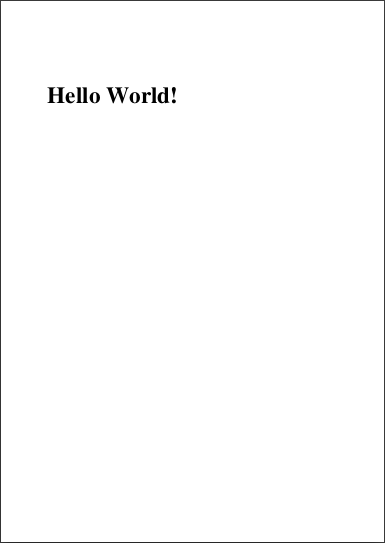
\includegraphics[width=0.6\textwidth,height=0.6\textheight,keepaspectratio]{figures/pshello.png}
\end{minipage}

\end{frame}

\begin{frame}[fragile,allowframebreaks]
\frametitle{Arquivos \texttt{.pdf} (Portable Document Format)}
PDF é uma evolução do PS. Ele é um formato de presentação de documento, ao invés de uma linguagem de programação.
Não é necessário um interpretator, bastando ler a descrição do documento.

\begin{lstlisting}[language=bash, label=lst-pdf, caption={Exemplo `Hello World!'.}, postbreak=\mbox{$\hookrightarrow$\space}, basicstyle=\fontsize{7}{9}\selectfont\ttfamily]
%PDF-1.4
1 0 obj <</Type /Catalog /Pages 2 0 R>>
endobj
2 0 obj <</Type /Pages /Kids [3 0 R] /Count 1>>
endobj
3 0 obj<</Type /Page /Parent 2 0 R /Resources 4 0 R /MediaBox [0 0 500 800] /Contents 6 0 R>>
endobj
4 0 obj<</Font <</F1 5 0 R>>>>
endobj
5 0 obj<</Type /Font /Subtype /Type1 /BaseFont /Times-Bold>>
endobj
6 0 obj
<</Length 44>>
stream
BT /F1 24 Tf 72 684 Td (Hello World!)Tj ET
endstream
endobj
xref
0 7
0000000000 65535 f
0000000009 00000 n
0000000056 00000 n
0000000111 00000 n
0000000212 00000 n
0000000250 00000 n
0000000317 00000 n
trailer <</Size 7/Root 1 0 R>>
startxref
406
%%EOF
\end{lstlisting}

\end{frame}



% arquivo .tex, .xml, .doc, docx, csv, xls, xlsx, png, jpg, pdf, etc
% tim hardfor podcast xls
\begin{frame}
\small
Sugestões de leitura:
\vspace{2ex}

\fullcite{harford2021}


\end{frame}

